\chapter{Training Neural Networks}

Until now, we saw various CNN architectures and the different layers that we can have in a model. But these models must also be trained, in order to obtain a working model. Here, we'll see various methods for training models, and the different tools that get used during training.

\section{Activation Functions}

Nowadays, there is a set of activation functions that are considered to be the avant-guarde of deep learning, but they might change in a few years. Although different, new versions and types of activation functions might come out, the reasoning between them remains mostly the same. But let's define first what an activation function is:

\begin{definition}{Activation Function}
    An \textbf{activation function} is a function which \textbf{determines} whether a given neuron should \textbf{activate} or not by computing the weighted sum $w$ and adding the bias $b$.
\end{definition}

Until now there are a lot of known and used activation functions: some of them are the \textbf{Sigmoid} function, the \textbf{ReLU}, etc... For now, we'll concentrate on the \textbf{sigmoid} activation function.

\begin{definition}{Sigmoid Activation Function}
    The \textbf{sigmoid activation function} is equal to
    \[ \sigma(x) \eq \frac{1}{1 + e^{-x}} \]

    The output of the sigmoid function is in the range $[0, \; 1]$.
\end{definition}

\noindent The sigmoid function was very popular back in the days, mainly because it represented very well when a neuron should "fire" or not. However, it has 3 main problems, which led to the abandonment of this function. The first problem is that \textbf{saturated neurons kill} the \textbf{gradient}. For instance, suppose that we have the following neuron:

\begin{center}
    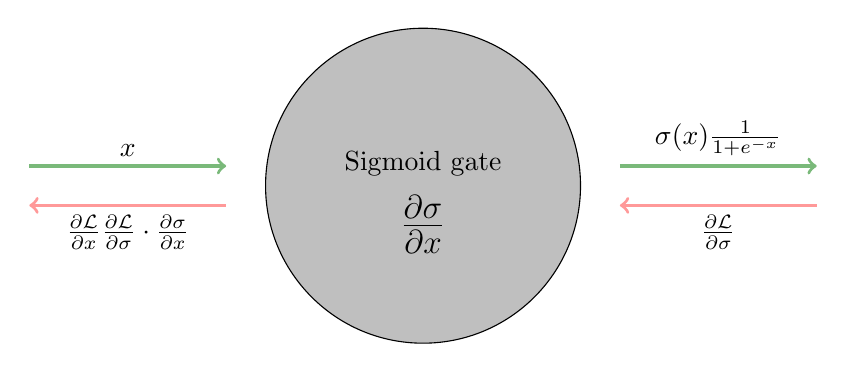
\begin{tikzpicture}
        \filldraw[gray!50, draw=black] (5, 1) circle (2cm) node [anchor = south] {\textcolor{black}{Sigmoid gate}};
        \draw[gray!50] (5, 1) circle (0.1pt) node [anchor = north] {\fontsize{18pt}{18pt}\selectfont\textcolor{black}{$\frac{\partial \sigma}{\partial x}$}};

        \draw[ForestGreen!60, very thick, ->] (0, 1.25) -- (2.5, 1.25);
        \draw[ForestGreen!60] (1.25, 1.25) circle (0.1pt) node [anchor = south] {\textcolor{black}{$x$}};
        \draw[red!40, very thick, <-] (0, 0.75) -- (2.5, 0.75); 
        \draw[red!40] (1.25, 0.75) circle (0.1pt) node [anchor = north] {\textcolor{black}{$\frac{\partial \mathcal{L}}{\partial x} \eq \frac{\partial \mathcal{L}}{\partial \sigma} \cdot \frac{\partial \sigma}{\partial x}$}};

        \draw[ForestGreen!60, very thick, ->] (7.5, 1.25) -- (10, 1.25);
        \draw[ForestGreen!60] (8.75, 1.25) circle (0.1pt) node [anchor = south] {\textcolor{black}{$\sigma(x) \eq \frac{1}{1 + e^{-x}}$}};
        \draw[red!40, very thick, <-] (7.5, 0.75) -- (10, 0.75); 
        \draw[red!40] (8.75, 0.75) circle (0.1pt) node [anchor = north] {\textcolor{black}{$\frac{\partial \mathcal{L}}{\partial \sigma}$}};
    \end{tikzpicture}
\end{center}

More specifically, we define the gradient of the sigmoid functions as follows:
\[ \frac{\partial \sigma}{\partial x} \eq \sigma(x) \cdot (1 - \sigma(x)) \]

Let us try to compute the value of the sigmoid gradient for 3 different values: for $10$, $0$ and $-10$. Let's begin with $x \eq 10$:
\[ \sigma(10) \eq \sim 0 \quad \quad \frac{\partial \sigma}{\partial x} \eq \sigma(10) \cdot (1 - \sigma(10)) \eq 0 \cdot (1 - 0) \eq 0 \]

Now, let's try with $x \eq 0$:
\[ \sigma(0) \eq 0,5 \quad \quad \frac{\partial \sigma}{\partial x} \eq \sigma(0) \cdot (1 - \sigma(0)) \eq 0,5 \cdot (1 - 0,5) \eq 0.25 \]

Finally, let's try with $x \eq -10$:
\[ \sigma(10) \eq \sim 1 \quad \quad \frac{\partial \sigma}{\partial x} \eq \sigma(10) \cdot (1 - \sigma(10)) \eq 1 \cdot (1 - 1) \eq 0 \]

We can see how the result of the gradient is mostly 0, and this clearly results in a problem because when the value of the gradient fill flow down into the network, then the parameters will never update.
\nl
The second problem with the sigmoid function is that the outputs of the sigmoid are \textbf{not centered in zero}.

\section{Data Preprocessing}

Generally the data can be 